\begin{frame}
\frametitle{Arquitectura del sistema}

\begin{itemize}
	\item<1-> \textcolor{UDCpink}{\itshape Front-end}: Creado en \textcolor{UDCpink}{LÖVE}, usa un modelo MVC que usa una interfaz gráfica en modo inmediato.
	
	\vspace{0.5em}
	
	\item<2-> \textcolor{UDCpink}{\itshape Back-end}: Creado en \textcolor{UDCpink}{Lua} (con API de clingo) y \textcolor{UDCpink}{ASP}, usa un modelo en \textit{pipeline}.
\end{itemize}

\pause[3]

\begin{center}
	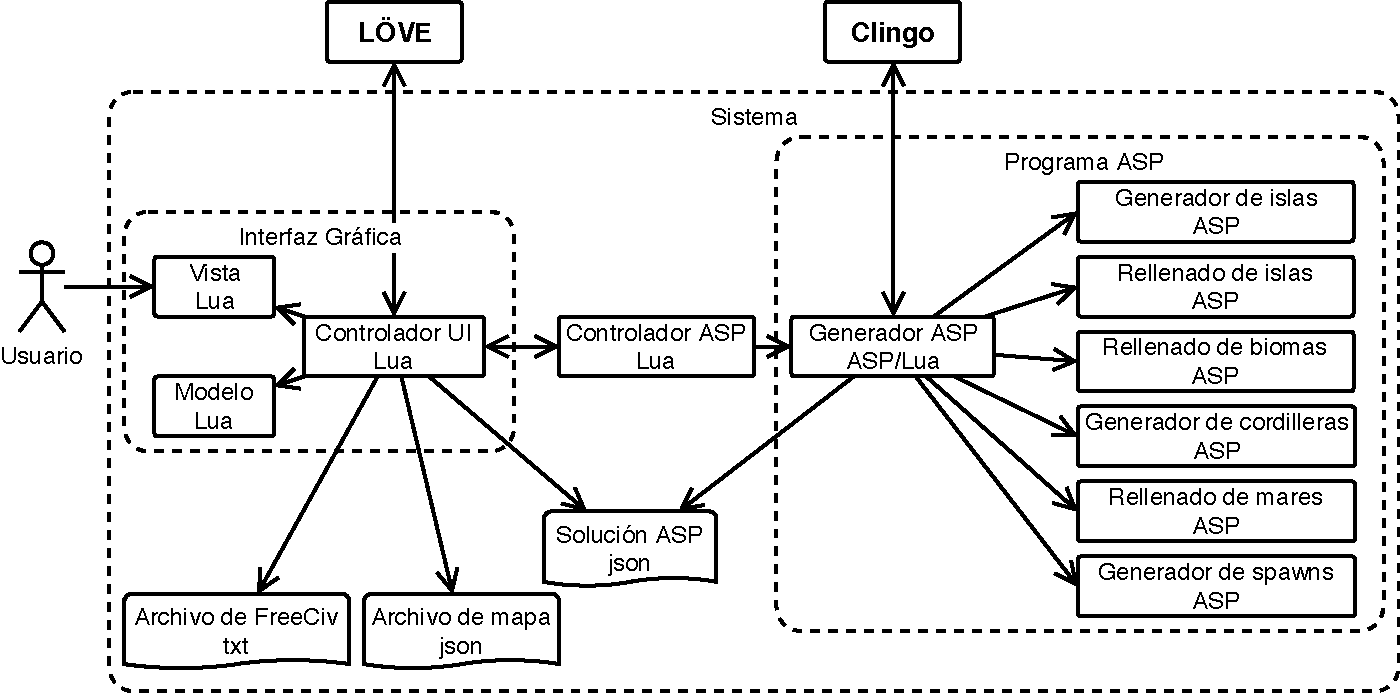
\includegraphics[width=.95\textwidth]{images/arquitectura-completa.pdf}
\end{center}

\end{frame}

\begin{frame}
\frametitle{Proceso de ingeniería}

\begin{itemize}
	\item<1-> Metodología: \textcolor{UDCpink}{desarrollo iterativo incremental y evolutivo}.
	
	\vspace{0.5em}
	
	\item<2-> Se ha usado herramientas de \textcolor{UDCpink}{uso libre y gratuitas} para el desarrollo del proyecto.
	
	\vspace{0.5em}
	
	\item<3-> El coste total del proyecto asciende a \textcolor{UDCpink}{\EUR{3720.00}}.
	
	\vspace{0.5em}	
\end{itemize}

\pause[4]

\centering
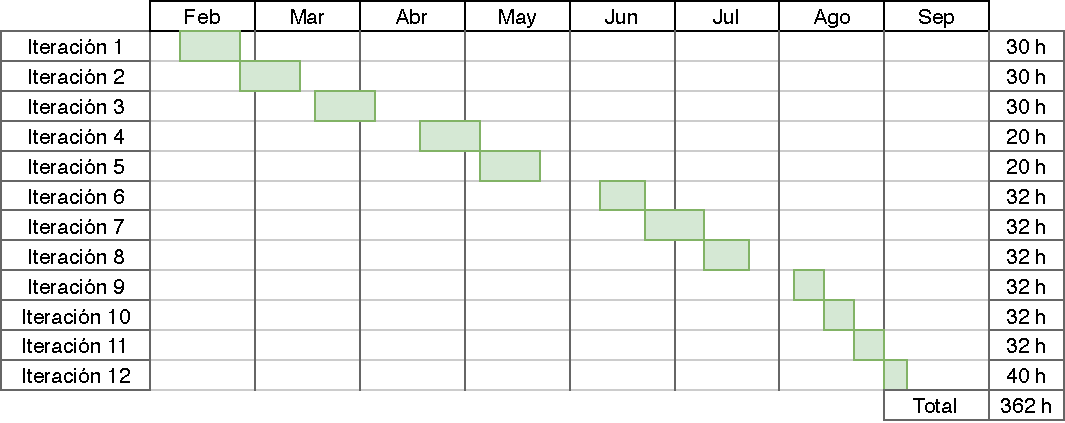
\includegraphics[width=\textwidth]{images/gantt.pdf}

\end{frame}